\documentclass[a4paper,12pt]{article} %
\usepackage[utf8]{inputenc} 
\usepackage[polish,english]{babel} 
\usepackage{graphicx}
\usepackage{hyperref} 
\usepackage{adjustbox} 
\usepackage{booktabs}
\usepackage{float}
\usepackage{siunitx} 
\usepackage[normalem]{ulem}
\useunder{\uline}{\ul}{}
\usepackage{geometry} 
\usepackage{titlesec} 
\usepackage{listings}
\usepackage{minted}
\usepackage{threeparttable}
\usepackage{multirow}

\titleformat{\section}{\normalfont\Large\bfseries}{\thesection.}{0.5em}{}
\titleformat{\subsection}{\normalfont\large\bfseries}{\thesubsection.}{0.5em}{}

\title{\textbf{Data Warehouse Optimization - Report}}
\author{Piotr Sulewski, Tomasz Sankowski}
\date{January 2025}

\begin{document}

\maketitle
\tableofcontents 
\newpage

\section{Aim of the Laboratory}
The aim of this task is to address issues related to various physical cube models and the design of aggregations. The focus is on demonstrating the impact of these models on performance and usability in a data warehouse environment.

\section{Preliminary Assumptions}

\subsection{Database Specifications}
\begin{itemize}
    \item \textbf{Size of the Data Warehouse:} 976.00 MB
    \item \textbf{Number of rows in the monitoring fact table (main):} 1,176,609
\end{itemize}

\subsection{Testing Environment}
Measurements were taken on the following setup:
\begin{itemize}
    \item \textbf{Processor:} Intel Core i7-6700K
    \item \textbf{Memory:} 16 GB RAM
    \item \textbf{Storage:} 1 TB NVMe SSD
    \item \textbf{Operating System:} Windows 10
    \item \textbf{Tools Used:}
    \begin{itemize}
        \item SQL Server Management Studio (SSMS) with SQL Server Profiler extension
        \item Visual Studio 2022 with Data Tools extension
    \end{itemize}
\end{itemize}

\subsection{Conditions During Testing}
To ensure reliable results, the following conditions were maintained:
\begin{itemize}
    \item Only the necessary applications were running during measurements:
    \begin{itemize}
        \item SQL Server Management Studio (SSMS)
        \item Visual Studio 2022
        \item A web browser with the instructions open
    \end{itemize}
\end{itemize}


\section{Theoretical Assumptions}

\begin{table}[H]
\centering
\caption{Comparison of MOLAP, HOLAP, and ROLAP}
\label{tab:comparison}
\begin{threeparttable}
\begin{tabular}{lccc}
\toprule
 & MOLAP & HOLAP & ROLAP \\
\midrule
\textbf{Querying time} & Short & Moderate\footnotemark[1] & Long \\
\textbf{Processing time} & Long & Moderate\footnotemark[2] & Short \\
\textbf{Total size} & Large\footnotemark[3] & Moderate & Small \\
\bottomrule
\end{tabular}
\begin{tablenotes}
\item[1] Querying time can be short if well-designed aggregations are used.
\item[2] Processing time is moderate, but if no aggregations are designed, it will be short.
\item[3] Total size can be smaller if no aggregations are designed for measure groups.
\end{tablenotes}
\end{threeparttable}
\end{table}


\newpage
\section{Testing}

\subsection{Brief description of the queries}
 Testing query execution times for different models, with and without defined aggregations.
 Testing cube processing times in the same testing settings
\begin{figure}[H]
    \caption{Query 2}
    \label{lst:query2}
    Which car models generate the highest earnings per vehicle?
    \begin{minted}{sql}
    WITH 
    MEMBER [Measures].[Vehicle Count] AS
        COUNT(EXISTING [Car].[Car ID].[Car ID])
    
    MEMBER [Measures].[Revenue Per Vehicle] AS
        IIF(
            [Measures].[Vehicle Count] > 0, 
            [Measures].[Rental Cost] / [Measures].[Vehicle Count], 
            NULL
        )
    
    SELECT 
        NON EMPTY 
        TOPCOUNT(
            [Car].[Brand].[Brand].MEMBERS *
    		[Car].[Model].[Model].MEMBERS,
            10, 
            [Measures].[Revenue Per Vehicle]
        ) ON ROWS,
        [Measures].[Revenue Per Vehicle] ON COLUMNS
    FROM 
        [Car Sharing];
    \end{minted}
\end{figure}

\begin{figure}[h]
    \caption{Query 5}
    \label{lst:query5}
Create a ranking of the 5 car models with the highest total mileage driven by customers in the last year.
    \begin{minted}{sql}
    SELECT 
    NON EMPTY
        TOPCOUNT(
    		[Car].[Brand].[Brand].MEMBERS *
            [Car].[Model].[Model].MEMBERS,
            5,
            [Measures].[Driven Km]
        ) ON ROWS,
        {[Measures].[Driven Km]} ON COLUMNS
    FROM 
        [Car Sharing]
    WHERE 
        ([Date].[DateHierarchy].[Year].&[2023]); 
    \end{minted}
\end{figure}

\begin{figure}[H]
    \caption{Query 9}
    \label{lst:query9}
Considering the number of rides taken and the number of reported damages, what is the theoretical probability of causing damage within each age group of users?
    \begin{minted}{sql}
    WITH
      MEMBER [Measures].[Damaged Rides] AS
        (
          [Was Damaged].[Was Damaged].[Damaged],
          [Measures].[Rental Count]
        )
      MEMBER [Measures].[Probability of Damage] AS
        IIF(
          [Measures].[Rental Count] = 0,
          null,
          [Measures].[Damaged Rides] / [Measures].[Rental Count]
        )
    SELECT
      { [Measures].[Probability of Damage] } ON COLUMNS,
      [User].[Age Category].Children ON ROWS
    FROM
      [Car Sharing];
    \end{minted}
\end{figure}


\subsection{MOLAP Performance}

\begin{table}[H]
\centering
\caption{Performance Comparison of MOLAP with and without Aggregators}
\label{tab:molap_performance}
\begin{tabular}{lcccccccc}
\toprule
& \multicolumn{8}{c}{MOLAP} \\
\cmidrule(lr){2-9}
& \multicolumn{4}{c}{Without Aggregators} & \multicolumn{4}{c}{With Aggregators} \\
\cmidrule(lr){2-9}
& Cube & Query & Query & Query & Cube & Query & Query & Query \\
& Processing & 2 & 5 & 9 & Processing & 2 & 5 & 9 \\
\midrule
& 4740 & 45 & 43 & 43 & 4910 & 4 & 2 & 2 \\
& 4635 & 43 & 46 & 44 & 4830 & 4 & 2 & 2 \\
& 4567 & 44 & 44 & 43 & 4907 & 4 & 3 & 3 \\
& 4732 & 45 & 43 & 44 & 4879 & 4 & 2 & 2 \\
& 4629 & 43 & 40 & 43 & 4867 & 4 & 5 & 1 \\
\midrule
Average & 4660.6 & 44 & 43.2 & 43.4 & 4878.6 & 4 & 2.8 & 2 \\
SD & 66.05 & 0.89 & 1.94 & 0.49 & 29.29 & 0.0 & 1.17 & 0.63 \\
\bottomrule
\end{tabular}
\end{table}

\subsection{HOLAP Performance}

\begin{table}[H]
\centering
\caption{Performance Comparison of HOLAP with and without Aggregators}
\label{tab:holap_performance}
\begin{tabular}{lcccccccc}
\toprule
& \multicolumn{8}{c}{HOLAP} \\
\cmidrule(lr){2-9}
& \multicolumn{4}{c}{Without Aggregators} & \multicolumn{4}{c}{With Aggregators} \\
\cmidrule(lr){2-9}
& Cube & Query & Query & Query & Cube & Query & Query & Query \\
& Processing & 2 & 5 & 9 & Processing & 2 & 5 & 9 \\
\midrule
& 483 & 141 & 135 & 301 & 513 & 5 & 2 & 2 \\
& 487 & 135 & 136 & 295 & 493 & 4 & 2 & 2 \\
& 479 & 136 & 150 & 299 & 498 & 5 & 2 & 1 \\
& 481 & 137 & 132 & 294 & 513 & 5 & 2 & 2 \\
& 482 & 132 & 163 & 316 & 558 & 4 & 2 & 1 \\
\midrule
Average & 482.4 & 136.2 & 143.8 & 301.0 & 515.0 & 4.6 & 2.0 & 1.6 \\
SD & 2.65 & 2.93 & 11.16 & 7.92 & 22.93 & 0.49 & 0.0 & 0.49 \\
\bottomrule
\end{tabular}
\end{table}

\subsection{ROLAP Performance}

\begin{table}[H]
\centering
\caption{Performance Comparison of ROLAP with and without Aggregators}
\label{tab:rolap_performance}
\begin{tabular}{lcccccccc}
\toprule
& \multicolumn{8}{c}{ROLAP} \\
\cmidrule(lr){2-9}
& \multicolumn{4}{c}{Without Aggregators} & \multicolumn{4}{c}{With Aggregators} \\
\cmidrule(lr){2-9}
& Cube & Query & Query & Query & Cube & Query & Query & Query \\
& Processing & 2 & 5 & 9 & Processing & 2 & 5 & 9 \\
\midrule
& 447 & 131 & 148 & 306 & 511 & 138 & 154 & 309 \\
& 526 & 135 & 142 & 307 & 566 & 139 & 137 & 305 \\
& 471 & 134 & 140 & 310 & 482 & 149 & 137 & 296 \\
& 487 & 137 & 151 & 299 & 499 & 133 & 139 & 323 \\
& 502 & 138 & 132 & 309 & 486 & 132 & 145 & 301 \\
\midrule
Average & 486.6 & 135.0 & 142.6 & 306.2 & 508.8 & 138.2 & 142.4 & 306.8 \\
SD & 26.84 & 2.45 & 6.62 & 3.87 & 30.37 & 6.05 & 6.50 & 9.17 \\
\bottomrule
\end{tabular}
\end{table}

\newpage
\subsection{Comparison of processing time for different cube models}
To achieve optimal results of the processing time of a cube we decided to take approximately 5 samples for each modification. The obtained results are presented in the following tables

\subsubsection{Comparison of cube processing performance}

\begin{table}[H]
\centering
\caption{Performance Comparison of Cube Processing with and without Aggregators in different cubes}
\label{tab:cube_processing_performance}
\begin{tabular}{@{}lcccccc@{}}
\toprule
\multirow{3}{*}{} & \multicolumn{6}{c}{Cube Processing} \\ \cmidrule(l){2-7} 
 & \multicolumn{3}{c|}{Without Aggregators} & \multicolumn{3}{c}{With Aggregators} \\ \cmidrule(l){2-7} 
 & MOLAP & HOLAP & \multicolumn{1}{c|}{ROLAP} & MOLAP & HOLAP & ROLAP \\ \midrule
\multicolumn{1}{c|}{Average} & 4660.6 & 482.4 & \multicolumn{1}{c|}{486.6} & 4878.6 & 515.0 & 508.8 \\
\multicolumn{1}{c|}{SD} & 66.05 & 2.65 & \multicolumn{1}{c|}{26.64} & 29.29 & 22.93 & 30.37
\end{tabular}
\end{table}

\subsubsection{Comparison of Query 2 performance}

\begin{table}[H]
\centering
\caption{Performance Comparison of Query 2 with and without Aggregators in different cubes}
\label{tab:query2_processing_performance}
\begin{tabular}{@{}lcccccc@{}}
\toprule
\multirow{3}{*}{} & \multicolumn{6}{c}{Query 2} \\ \cmidrule(l){2-7} 
 & \multicolumn{3}{c|}{Without Aggregators} & \multicolumn{3}{c}{With Aggregators} \\ \cmidrule(l){2-7} 
 & MOLAP & HOLAP & \multicolumn{1}{c|}{ROLAP} & MOLAP & HOLAP & ROLAP \\ \midrule
\multicolumn{1}{c|}{Average} & 44.0 & 136.2 & \multicolumn{1}{c|}{135.0} & 4.0 & 4.6 & 138.2 \\
\multicolumn{1}{c|}{SD} & 0.89 & 2.93 & \multicolumn{1}{c|}{2.45} & 0.0 & 0.49 & 6.05
\end{tabular}
\end{table}

\subsubsection{Comparison of Query 5 performance}

\begin{table}[H]
\centering
\caption{Performance Comparison of Query 5 with and without Aggregators in different cubes}
\label{tab:query5_processing_performance}
\begin{tabular}{@{}lcccccc@{}}
\toprule
\multirow{3}{*}{} & \multicolumn{6}{c}{Query 5} \\ \cmidrule(l){2-7} 
 & \multicolumn{3}{c|}{Without Aggregators} & \multicolumn{3}{c}{With Aggregators} \\ \cmidrule(l){2-7} 
 & MOLAP & HOLAP & \multicolumn{1}{c|}{ROLAP} & MOLAP & HOLAP & ROLAP \\ \midrule
\multicolumn{1}{c|}{Average} & 43.2 & 143.8 & \multicolumn{1}{c|}{142.6} & 2.8 & 2.0 & 142.4 \\
\multicolumn{1}{c|}{SD} & 1.94 & 11.6 & \multicolumn{1}{c|}{6.62} & 1.17 & 0.0 & 6.50
\end{tabular}
\end{table}

\subsubsection{Comparison of Query 9 performance}
\begin{table}[H]
\centering
\caption{Performance Comparison of Query 9 with and without Aggregators in different cubes}
\label{tab:query5_processing_performance}
\begin{tabular}{@{}lcccccc@{}}
\toprule
\multirow{3}{*}{} & \multicolumn{6}{c}{Query 9} \\ \cmidrule(l){2-7} 
 & \multicolumn{3}{c|}{Without Aggregators} & \multicolumn{3}{c}{With Aggregators} \\ \cmidrule(l){2-7} 
 & MOLAP & HOLAP & \multicolumn{1}{c|}{ROLAP} & MOLAP & HOLAP & ROLAP \\ \midrule
\multicolumn{1}{c|}{Average} & 43.4 & 301.0 & \multicolumn{1}{c|}{306.2} & 2.0 & 1.6 & 306.8 \\
\multicolumn{1}{c|}{SD} & 0.49 & 7.92 & \multicolumn{1}{c|}{3.87} & 0.63 & 0.49 & 9.17
\end{tabular}
\end{table}

\newpage
\section{Cache and Aggregation Settings}
\subsection{Aggregation Design}
The aggregations were designed with the “Perforfamous gain reaches” option set to 100\%, which gave us 7 aggregations with an optimization level of 40\% (4.4MB).
\begin{figure}[H]
    \centering
    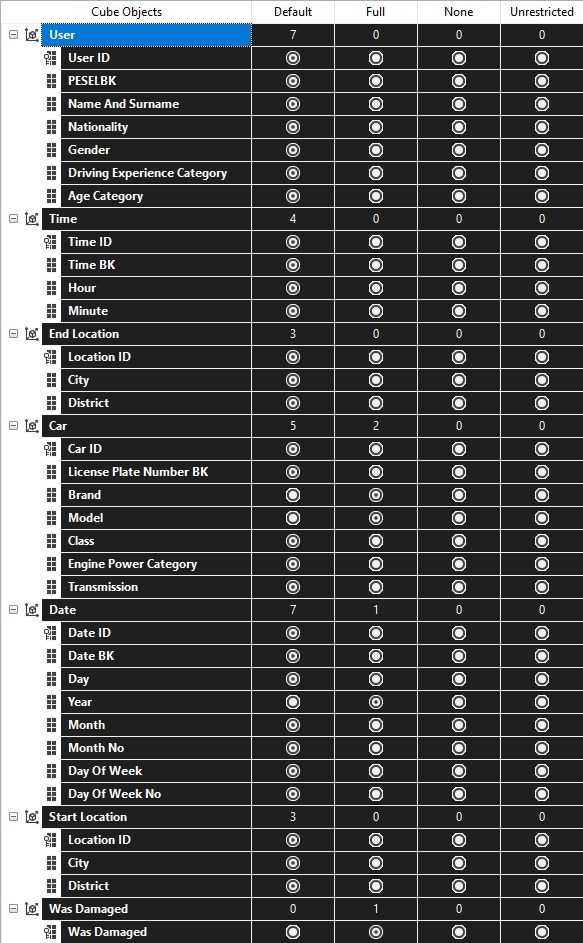
\includegraphics[width=0.5\linewidth]{aggregation_design.jpg}
    \caption{Aggregation Usage}
    \label{fig:aggregation-usage}
\end{figure}
\subsection{Cache removal}
\begin{figure}[H]
    \caption{Cache}
    \label{lst:cache}
Removing cache
\begin{minted}{xml}
<ClearCache xmlns="http://schemas.microsoft.com/analysisservices/2003/engine">
    <Object>
        <DatabaseID>CarSharingImplementation</DatabaseID>
    </Object>
</ClearCache>
\end{minted}
\end{figure}

\newpage
\section{Discussion}

\subsection{Cube Processing}
As observed, MOLAP required nearly ten times more time to process the cube compared to the ROLAP and HOLAP approaches, both with and without aggregations. This is because the MOLAP server needed to copy the entire warehouse storage into the cube, significantly slowing down the processing time. Additionally, adding aggregations only slightly affected the cube processing time, increasing it by approximately 10\%. The higher processing time is due to the need to group measures by dimension members during cube processing. Our results confirm the assumption that MOLAP's cube processing time is considerably slower than ROLAP's and HOLAP's.

\subsection{Query Execution}
MOLAP query execution was, on average and depending on the specific query, 3 to 8 times faster than executing queries on the ROLAP server. The query execution time on the HOLAP server was similar to that of ROLAP. This supports our assumption that, despite requiring more time for cube processing, the MOLAP server significantly outperforms the other types of data warehouses in query execution because it already contains the necessary data within the cube.

Moreover, adding aggregations had no noticeable effect on the ROLAP server's query execution time. However, it made MOLAP and HOLAP almost equally efficient, with aggregations speeding up MOLAP query execution by about 20 times and HOLAP by approximately 70 to 150 times. This highlights the effectiveness of using aggregations. Aggregations accelerate query execution because the cube doesn't need to spend time grouping measures by dimension attributes; this grouping is already done during cube processing. HOLAP's query execution time was significantly better because, during the cube processing, aggregations are transferred to the cube, eliminating the need to retrieve data from the relational warehouse during aggregation.

\newpage

\subsection{General Conclusions}
The tests on MOLAP, ROLAP, and HOLAP reveal key performance differences:

\begin{enumerate}
    \item \textbf{Cube Processing Time:} MOLAP is slower to process the cube, as it requires transferring data into the multidimensional structure. ROLAP, however, directly accesses the relational database, making it faster. HOLAP offers a hybrid approach, with performance similar to ROLAP.
    
    \item \textbf{Query Execution Time:} MOLAP accelerates query execution by storing data in the cube, significantly outperforming ROLAP. HOLAP, with aggregations, also sees major query performance improvements, as aggregated data is stored within the cube, bypassing the need for relational data access.
    
    \item \textbf{Impact of Aggregations:} Adding aggregations enhances query performance in MOLAP and HOLAP, reducing query time by eliminating the need for grouping measures during execution. ROLAP shows no improvement as it still relies on the relational database for query execution.
    
    \item \textbf{Overall Performance:} MOLAP excels in query speed but has slower processing times. ROLAP is faster for cube processing but slower in query execution. HOLAP offers a balanced solution, with faster query performance when aggregations are used, making it ideal for systems requiring both efficient data storage and quick queries.
\end{enumerate}

In conclusion, the choice between OLAP models depends on specific needs: MOLAP is best for fast queries, ROLAP for quicker processing, and HOLAP offers a middle ground.

\end{document}
